\chapter{Hardware versus Software}

In the preceding weeks we've learned about hardware, the physical components that make up computing
systems. Hardware is only half of what constitute computing systems. Software is the ``brain'' of
a computer system that dictates how the hardware should execute. Hardware without software is like
a car without a driver --- it is unable to do much. Similarly, software without hardware to run on
is like a driver without a car, it has nothing to drive. Together software and hardware are able to
perform work in a meaningful and controlled way.

In this section, we will discuss the distinction between hardware and software and how they
interact. As seen in Figure~\ref{fig:hw_sw:layers}, many layers of software sit between the hardware of
our computer systems and the software we use and develop. These layers build up from the hardware and
abstract away many of the complexities of lower levels to provide more and more functionality.

\begin{figure}
\centering
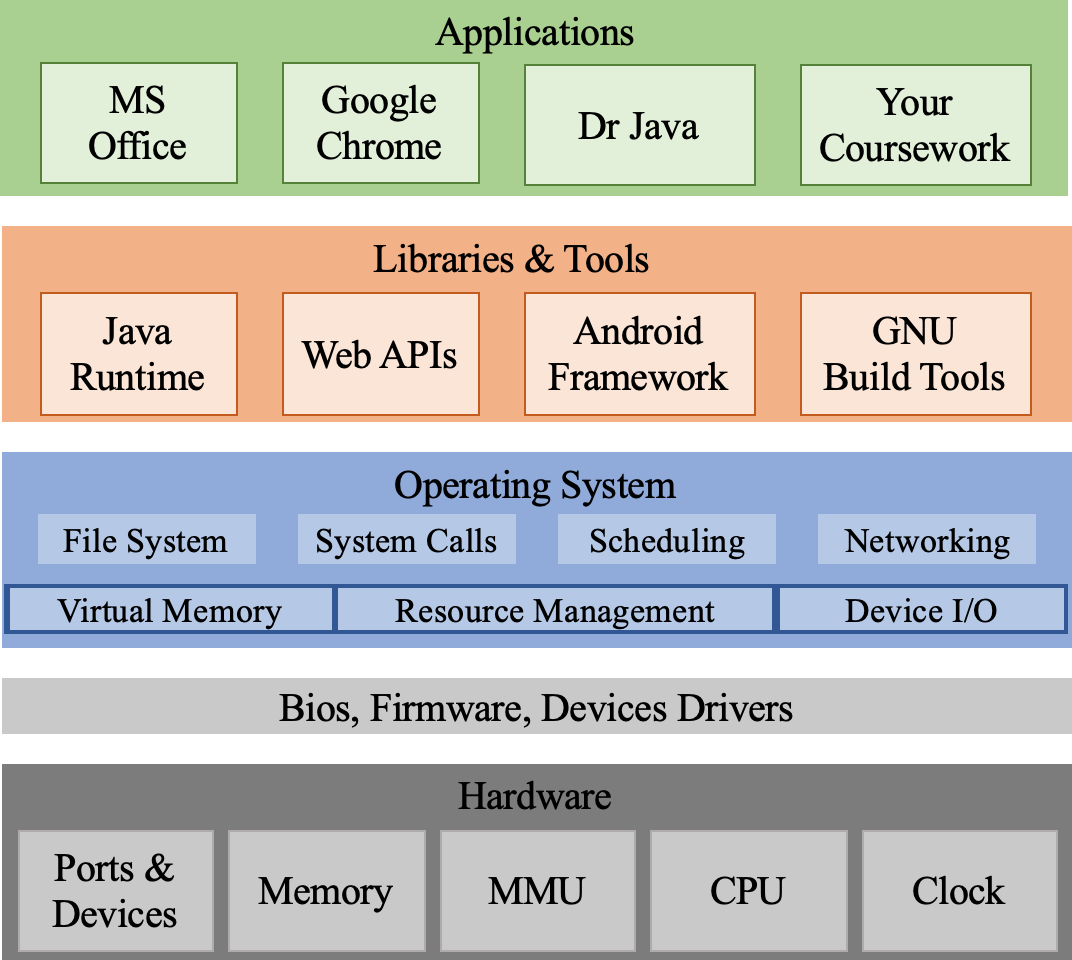
\includegraphics[width=6.5cm]{images/software_layers.png}
\caption{Layers of software built up from hardware. Each providing more abstractions and functionality for higher levels to use.}
\label{fig:hw_sw:layers}
\end{figure}

\section{Hardware}
As discussed previously, hardware is the collection of physical devices that make up a computer.
The hardware performs the actual computations by manipulating electrical currents. Today most
computers are digital, meaning that the computer works by representing data with electrical currents
at a High or Low voltage. We think of these high-voltages at representing on or 1 and low-voltages
as off or 0. The only thing the hardware understands are these voltages. However, there is a direct
translation from these voltages to binary numbers. This representation as binary numbers is often
called the computer's machine language. Not all computers recognize the same machine code language ---
the same sequence of 1's and 0's may not represent the same information on two computers ---
and is often manufacturer dependent.

Often times, manufacturers of computers (more specifically manufacturers of central processing units)
describe what machine language a computer understands by providing another language called
an assembly language. This assembly language has a one-to-one translation to machine code language.
This assembly language is designed to be more human-readable than machine code. (e.g. \ic{store x0 M(x1)1000}
as opposed to 01100100000000011000, where both mean store the value of register \ic{x0} into the memory location
offset by 1000 from the location pointed at by register ic{x1}). While each computer manufacturer may
have their own machinge code for each computer they design, there are far fewer assembly languages.
Today, the most popular assembly languages include MIPS, ARM, RISC-V, and Intel x64. With assembly
languages, computer manufacturers only need to supply the translation from assembly language
to their machine code (and thus into high and low voltages).

\section{BIOS and Firmware}
Today, it is very likely that the first software loaded onto any computing device is a firmware.
Firmware is software that helps facilitate other software interacting with the computer device.
One notable piece of firmware is called the BIOS (Basic Input/Output System). You would be hard-pressed
to find any personal computer or smartphone that doesn't have a BIOS already pre-installed by
the device's manufacturer. A BIOS helps facilitate initial loading of programs onto a computer.
A BIOS will tell the computer to look for a connected device trying to communicate with the
computer (e.g. CD or USB drives). 

\begin{figure}
    \centering
    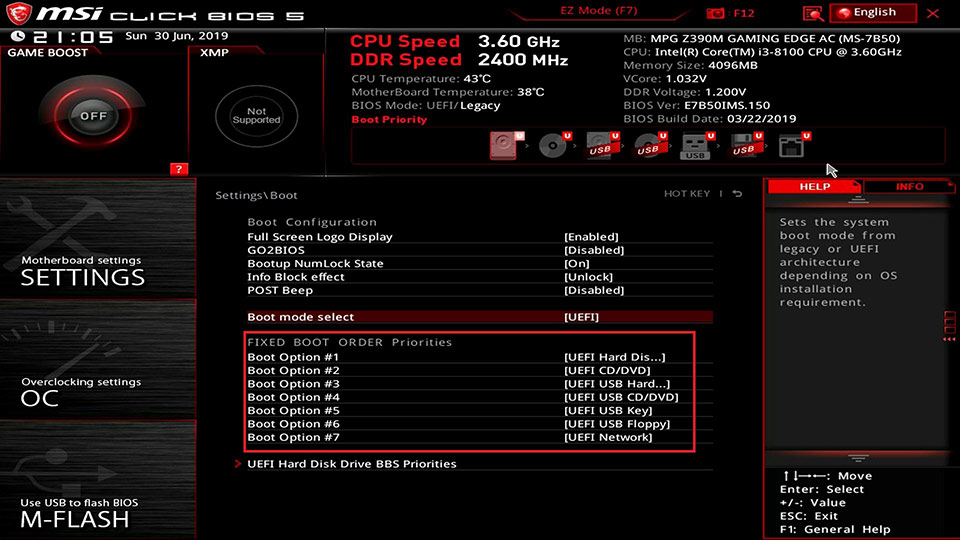
\includegraphics[width=12cm]{images/bios.jpg}
    \caption{Layers of software built up from hardware. Each providing more abstractions and functionality for higher levels to use.}
    \label{fig:hw_sw:bios}
\end{figure}

Figure \ref{fig:hw_sw:bios} shows a relatively modern and user-friendly BIOS interface, with the settings
for boot order highlighted. In this instance, the BIOS is set to first boot from an operating system
on the hard disk, if one is available. This is the typical scenario for a computer which has already
been set up. If there is no operating system on the hard disk, the BIOS is configured to try to boot
from a CD or a USB drive instead. These devices might be used to initially install the operating system.

\section{Operating Systems}
Today it is very hard to find any personal device that doesn't come pre-installed with an
operating system, and if it does the first thing you'll do is install an operating system
onto it. Today the most popular operating systems include MacOS, Windows, Linux, or
various flavors of each. The operating system handles all of the low-level details of the
computer, manages computing resources, and exposes a high-level interface that user-programs
may use. In this sense, the operating system of a computer is like the subconscious parts
of our brain. Things like file systems, memory management, processes, threads, scheduling,
user programs, kernel programs, and system calls are all designed and implemented by the
operating system. When a user decides to run a program, the operating system will start
the program and hand over control to the program for some time.

Generally speaking, the operating system is in charge of how to properly run all the
programs the user wants to run. The operating system will handle how to manage
shared resources (memory, CPU-time, input and output devices). These resources are often
requested by programs through the use of system calls.
These system calls switch control from the program to the operating system,
so that the operating system can execute on the programs behalf and help
distribute the shared resources accordingly.

\section{Libraries and Tools}
There are many repeated designs and functionalities that programmers
want to use. For example, many applications may need to include a clickable
button. Even things you might not even think about can be tricky. For example,
writing a program to display the current time in a user's timezone is quite complex,
due to overlapping and conflicting standards for timezone offsets and Daylight Saving Time.
Instead of every programmer and program including their own
version of these repeated designs and code. These are provided to the
end programmer in the forms of tools and libraries. A library is
similar to the system calls provided by the operating system. A library
provides an interface that the programmer can use to have the library
execute code on a program's behalf. Libraries offer a plethora of
functionality including thread-safe data structures, networking
APIs, graphics functions, and many more. Tools are very similar
but instead are their own program that one can interact with
rather than use it as a programming interface. Tools range
from the simple (a text editor, or a program to view the file system)
to the complex (such as Integrated Development Environments or IDEs, such as Dr. Java).

\section{Applications}
On top of all of these, sits user programs. These are the programs that
an end user will run, and that you yourself may write. These build upon
all of the functionality provided by the operating systems, tools,
and libraries to build new and novel applications. There are a limitless
number of applications that you can create by using the resources
available for programmers. Today, popular applications include mobile games,
browsers, word processors, messaging apps, and much more.

\section{Java Virtual Machine}

For a long time, the model shown in Figure \ref{fig:hw_sw:layers} worked well. A program written in an old language, such as C, would be compiled. The compiler would translate the programmer's C code into assembly language, and then the assembly code could be run on the programmer's computer. If the programmer wanted the program to run on a computer with a different assembly language, they could compile their program with a compiler written for that assembly language, and distribute that version of the compiled code accordingly.

This changed when the Internet was created. Suddenly, instead of sending floppy disks or CD-ROMs in the mail to specific intended users, it became possible -- in principle -- to distribute a program broadly by making it available on the Internet. However, since the end user could be using a computer which understands one of many possible assembly languages, the programmer would have to make many different versions of the program available. Even if the programmer could compile her program for every possible assembly language, the user would have to know which version to download, which could be difficult.

Java was created largely to address this issue. When you compile a Java program, you get a \ic{.class} file, which cannot be executed directly by your computer. Instead, you run \ic{java MyClass.class}, which loads a program called the Java Virtual Machine, or JVM. The JVM essentially simulates a computer with a fixed assembly language. When you downloaded the Java Development Kit, part of it was a tool called the Java Runtime Environment which operates the JVM. This way, there is only one way to compile a Java program: you run \ic{javac} and produce a \ic{.class} file. You could put this \ic{.class} file on the Internet, and another Java user could download it and run it on their JVM. The only computer-specific software is the JVM itself, which is available for any kind of computer.